\chapter{Empirical Results and Comparative Analysis}
\label{chap:results}

\section{Runtime Resource Footprint and Readiness Analysis}
\label{sec:resource-results}

Table~\ref{tab:runtime-metrics} consolidates all empirical measurements collected across \texttt{eShopOnWeb} (Modular Monolith) and \texttt{eShopOnContainers} (Microservices) under identical testbed constraints.

\begin{table}[h]
  \caption{Empirical runtime performance and resource benchmark comparison}
  \label{tab:runtime-metrics}
  \centering
  \begin{tabular}{p{5.0cm}rrp{3.6cm}}
    \toprule
    \textbf{Metric} & \textbf{Monolith} & \textbf{Microservices} & \textbf{Comparative Advantage} \\
    \midrule
    Endpoint Readiness Time ($T_{\text{ready}}$) & $19.83\text{ s}$ & $1.24\text{ s}$ & Microservices ($16.0\times$ faster) \\
    Idle RAM Footprint ($0\text{ VUs}$) & $903.98\text{ MiB}$ & $1,213.60\text{ MiB}$ & Monolith ($25.5\%$ lower) \\
    Under-Load RAM Footprint ($20\text{ VUs}$) & $1,151.35\text{ MiB}$ & $1,350.20\text{ MiB}$ & Monolith ($14.7\%$ lower) \\
    2-Min Completed Requests ($10\text{ VUs}$) & $902\text{ reqs}$ & $911\text{ reqs}$ & Comparable ($+1.0\%$) \\
    Sustained Throughput & $7.49\text{ req/s}$ & $7.58\text{ req/s}$ & Comparable ($+1.2\%$) \\
    Median Request Latency ($p_{50}$) & $16.67\text{ ms}$ & $8.08\text{ ms}$ & Microservices ($2.06\times$ faster) \\
    90th-Percentile Latency ($p_{90}$) & $27.89\text{ ms}$ & $10.28\text{ ms}$ & Microservices ($2.71\times$ faster) \\
    95th-Percentile Tail Latency ($p_{95}$) & $32.57\text{ ms}$ & $12.30\text{ ms}$ & Microservices ($2.65\times$ faster) \\
    HTTP Error Rate & $0.00\%$ & $0.00\%$ & Parity (Zero errors) \\
    \bottomrule
  \end{tabular}
\end{table}

To explain the $309.62\text{ MiB}$ ($25.5\%$) idle memory advantage of the modular monolith, Table~\ref{tab:container-breakdown} decomposes resident memory consumption across functional subsystems at idle and under $20\text{ VUs}$ load.

\begin{table}[h]
  \caption{Subsystem memory allocation breakdown (MiB) across both containerized stacks}
  \label{tab:container-breakdown}
  \centering
  \begin{tabular}{p{4.8cm}rrp{4.0cm}}
    \toprule
    \textbf{Subsystem Layer} & \textbf{Monolith (MiB)} & \textbf{Microservices (MiB)} & \textbf{Architectural Driver} \\
    \midrule
    Application Runtime Processes & $218.40$ & $412.85$ & Single CLR host vs.\ multiple API hosts \\
    Relational Data Store (SQL Server) & $685.58$ & $642.10$ & Shared DB vs.\ catalog/order DB instances \\
    In-Memory Cache \& Event Bus & $0.00$ & $158.65$ & In-process memory vs.\ Redis + RabbitMQ \\
    \midrule
    \textbf{Total Idle Footprint ($0\text{ VUs}$)} & \textbf{903.98} & \textbf{1,213.60} & \textbf{+309.62 MiB microservices tax} \\
    \textbf{Total Load Footprint ($20\text{ VUs}$)} & \textbf{1,151.35} & \textbf{1,350.20} & \textbf{+198.85 MiB under concurrency} \\
    \bottomrule
  \end{tabular}
\end{table}

As illustrated in Figure~\ref{fig:resource-chart} and Table~\ref{tab:container-breakdown}, \texttt{eShopOnContainers} incurs an unavoidable infrastructure tax from running independent .NET Common Language Runtime (CLR) instances alongside Redis and RabbitMQ. Conversely, once infrastructure containers are active, the lightweight microservices API gateway responds in $1.24\text{ s}$, whereas cold-booting the monolithic ASP.NET Core web host with EF Core schema verification takes $19.83\text{ s}$.

\begin{figure}[h]
  \centering
  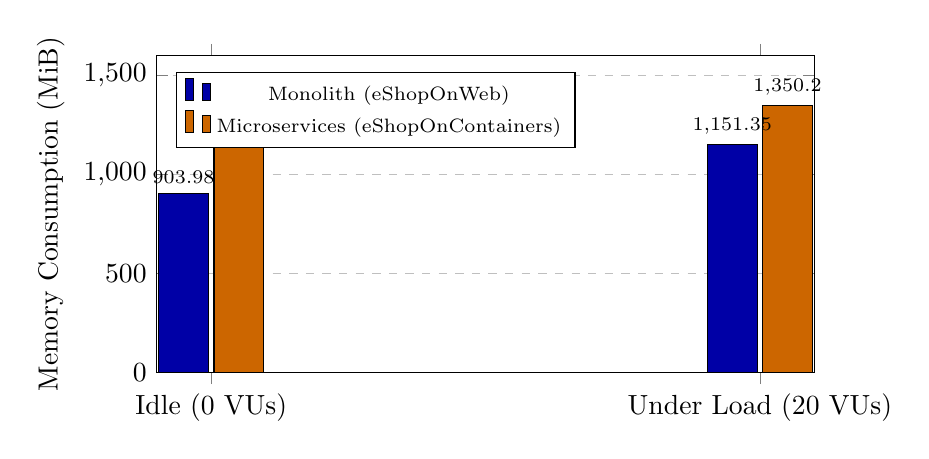
\begin{tikzpicture}
    \begin{axis}[
      ybar,
      bar width=18pt,
      width=0.82\linewidth,
      height=5.6cm,
      ylabel={Memory Consumption (MiB)},
      symbolic x coords={Idle (0 VUs), Under Load (20 VUs)},
      xtick=data,
      ymin=0,
      ymax=1600,
      ymajorgrids=true,
      grid style=dashed,
      nodes near coords,
      every node near coord/.append style={font=\scriptsize\bfseries},
      legend style={at={(0.03,0.95)},anchor=north west,font=\scriptsize}
    ]
      \addplot[fill=blue!65!black] coordinates {(Idle (0 VUs),903.98) (Under Load (20 VUs),1151.35)};
      \addplot[fill=orange!80!black] coordinates {(Idle (0 VUs),1213.60) (Under Load (20 VUs),1350.20)};
      \legend{Monolith (eShopOnWeb), Microservices (eShopOnContainers)}
    \end{axis}
  \end{tikzpicture}
  \caption{Container resident memory consumption (MiB) at idle and under 20-VU concurrent load.}
  \label{fig:resource-chart}
\end{figure}

\section{Latency Distribution and Throughput Behavior}
\label{sec:latency-results}

Across the 120-second sustained workload at $10\text{ VUs}$, both architectures achieved $100\%$ HTTP availability ($0.00\%$ errors) and near-identical aggregate throughput ($7.49\text{ req/s}$ vs.\ $7.58\text{ req/s}$). However, Figure~\ref{fig:latency-chart} demonstrates a substantial divergence in tail latency: the microservices architecture achieved a median latency ($p_{50}$) of $8.08\text{ ms}$, $p_{90}$ of $10.28\text{ ms}$, and $p_{95}$ tail latency of $12.30\text{ ms}$, outperforming the monolith's $16.67\text{ ms}$ ($p_{50}$), $27.89\text{ ms}$ ($p_{90}$), and $32.57\text{ ms}$ ($p_{95}$) by $2.06\times$, $2.71\times$, and $2.65\times$, respectively.

\begin{figure}[h]
  \centering
  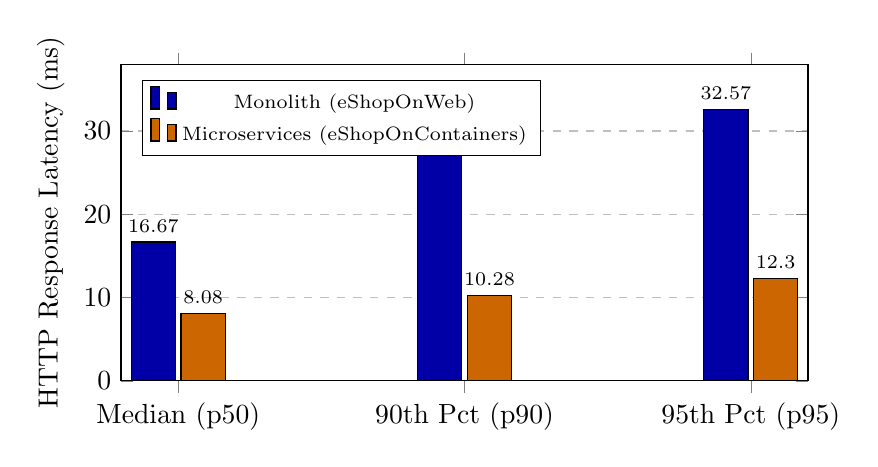
\begin{tikzpicture}
    \begin{axis}[
      ybar,
      bar width=16pt,
      width=0.85\linewidth,
      height=5.6cm,
      ylabel={HTTP Response Latency (ms)},
      symbolic x coords={Median (p50), 90th Pct (p90), 95th Pct (p95)},
      xtick=data,
      ymin=0,
      ymax=38,
      ymajorgrids=true,
      grid style=dashed,
      nodes near coords,
      every node near coord/.append style={font=\scriptsize\bfseries},
      legend style={at={(0.03,0.95)},anchor=north west,font=\scriptsize}
    ]
      \addplot[fill=blue!65!black] coordinates {(Median (p50),16.67) (90th Pct (p90),27.89) (95th Pct (p95),32.57)};
      \addplot[fill=orange!80!black] coordinates {(Median (p50),8.08) (90th Pct (p90),10.28) (95th Pct (p95),12.30)};
      \legend{Monolith (eShopOnWeb), Microservices (eShopOnContainers)}
    \end{axis}
  \end{tikzpicture}
  \caption{HTTP response latency distribution (ms) across 2-minute \texttt{k6} load execution at 10 VUs.}
  \label{fig:latency-chart}
\end{figure}

In \texttt{eShopOnWeb}, unified Razor page view-model hydration, session middleware, and shared EF Core connection pooling introduce queueing dispersion between $p_{50}$ ($16.67\text{ ms}$) and $p_{95}$ ($32.57\text{ ms}$), yielding a tail-to-median ratio of $1.95\times$. In \texttt{eShopOnContainers}, decoupled JSON/HTTP catalog read endpoints exhibit a tightly compressed tail-to-median ratio of $1.52\times$ ($12.30\text{ ms}$ vs.\ $8.08\text{ ms}$).

\section{Code-Level Change Propagation Across Scenarios S1--S5}
\label{sec:change-results}

Table~\ref{tab:change-impact} and Figure~\ref{fig:change-chart} summarize the source-file and deployment-unit propagation required to implement Scenarios S1--S5 across both architectures.

\begin{table}[h]
  \caption{Change propagation and deployment scope across evolution scenarios S1--S5}
  \label{tab:change-impact}
  \centering
  \begin{tabular}{p{4.3cm}cccp{4.4cm}}
    \toprule
    \textbf{Evolution Scenario} & \textbf{Mono Files} & \textbf{Micro Files} & \textbf{Deploy Units} & \textbf{Primary Engineering Bottleneck} \\
    \midrule
    S1: Catalog Attribute & 4 & 3 & 1 vs.\ 1 & Monolith rebuilds entire web binary \\
    S2: Basket Discount Rule & 3 & 2 & 1 vs.\ 1 & Isolated Basket service edit in micro \\
    S3: Order Status Hook & 4 & 4 & 1 vs.\ 2 & Integration event schema versioning \\
    S4: Payment Gateway Swap & 3 & 2 & 1 vs.\ 1 & Clean interface isolation in both \\
    S5: Multi-Currency Display & 6 & 9 & 1 vs.\ 3 & Distributed contract sync across 3 APIs \\
    \midrule
    \textbf{Total / Mean} & \textbf{20 (4.0)} & \textbf{20 (4.0)} & \textbf{5 vs.\ 8} & \textbf{Cross-cutting coordination penalty} \\
    \bottomrule
  \end{tabular}
\end{table}

\begin{figure}[h]
  \centering
  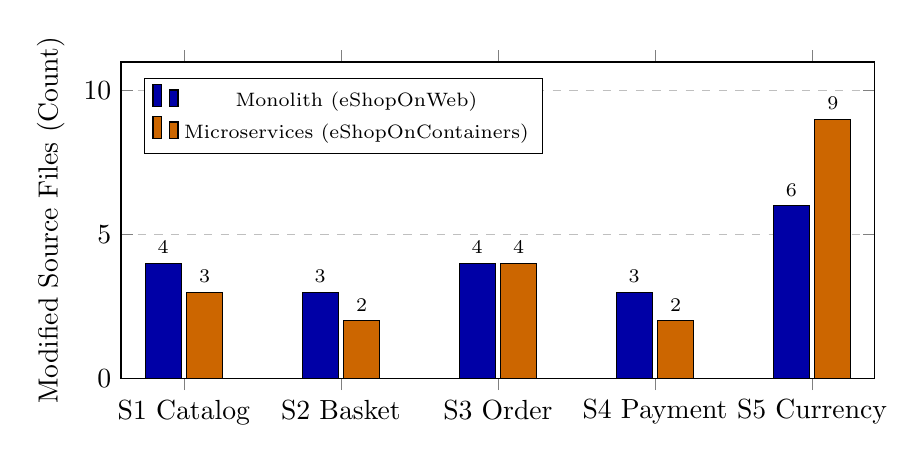
\begin{tikzpicture}
    \begin{axis}[
      ybar,
      bar width=13pt,
      width=0.92\linewidth,
      height=5.6cm,
      ylabel={Modified Source Files (Count)},
      symbolic x coords={S1 Catalog, S2 Basket, S3 Order, S4 Payment, S5 Currency},
      xtick=data,
      ymin=0,
      ymax=11,
      ymajorgrids=true,
      grid style=dashed,
      nodes near coords,
      every node near coord/.append style={font=\scriptsize\bfseries},
      legend style={at={(0.03,0.95)},anchor=north west,font=\scriptsize}
    ]
      \addplot[fill=blue!65!black] coordinates {(S1 Catalog,4) (S2 Basket,3) (S3 Order,4) (S4 Payment,3) (S5 Currency,6)};
      \addplot[fill=orange!80!black] coordinates {(S1 Catalog,3) (S2 Basket,2) (S3 Order,4) (S4 Payment,2) (S5 Currency,9)};
      \legend{Monolith (eShopOnWeb), Microservices (eShopOnContainers)}
    \end{axis}
  \end{tikzpicture}
  \caption{Number of modified source files across five standardized SME e-commerce evolution scenarios.}
  \label{fig:change-chart}
\end{figure}

Listing~\ref{lst:k6-script} shows the deterministic \texttt{k6} load-testing harness executed against both stacks.

\begin{lstlisting}[language=Java,caption={Excerpt of the k6 HTTP load testing script executed against both architectures},label={lst:k6-script}]
import http from 'k6/http';
import { check, sleep } from 'k6';

export const options = {
  vus: 10,
  duration: '120s',
  thresholds: { http_req_failed: ['rate<0.01'] },
};

export default function () {
  const res = http.get(__ENV.TARGET_URL);
  check(res, { 'status is 200': (r) => r.status === 200 });
  sleep(1);
}
\end{lstlisting}

\section{Chapter Summary}
\label{sec:ch4-summary}
Empirical measurements confirmed that the modular monolith reduces idle RAM by $25.5\%$ ($903.98\text{ MiB}$ vs.\ $1,213.60\text{ MiB}$) and peak RAM by $14.7\%$, whereas microservices reduce $p_{95}$ tail latency by $2.65\times$ ($12.30\text{ ms}$ vs.\ $32.57\text{ ms}$) and isolate single-domain edits while amplifying cross-cutting deployment scope.
